% Created 2021-09-11 Sat 20:47
% Intended LaTeX compiler: pdflatex
\documentclass{scrartcl}
\usepackage[utf8]{inputenc}
\usepackage[T1]{fontenc}
\usepackage{fontspec}
\usepackage{graphicx}
\usepackage{grffile}
\usepackage{longtable}
\usepackage{wrapfig}
\usepackage{rotating}
\usepackage[normalem]{ulem}
\usepackage{amsmath}
\usepackage{textcomp}
\usepackage{amssymb}
\usepackage{capt-of}
\usepackage[dvipsnames]{xcolor}
\usepackage[colorlinks=true, linkcolor=Blue, citecolor=BrickRed, urlcolor=PineGreen]{hyperref}
\usepackage{indentfirst}
\setmainfont[Ligatures=TeX]{Alegreya}
\setmonofont[Ligatures=TeX]{Liga SFMono Nerd Font}
\usepackage{chemfig}
\usepackage[version=4]{mhchem}

% features: (acronym underline par-sep)
\newcommand{\acr}[1]{\protect\textls*[110]{\scshape #1}}
\newcommand{\acrs}{\protect\scalebox{.91}[.84]\hspace{0.15ex}s}
\usepackage[normalem]{ulem}
\setlength{\parskip}{\baselineskip}
\setlength{\parindent}{0pt}

% end features

%% make document follow Emacs theme

\definecolor{obg}{HTML}{fafafa}
\definecolor{ofg}{HTML}{383a42}

\pagecolor{obg}
\color{ofg}

% list labels

\definecolor{itemlabel}{HTML}{4078f2}

\renewcommand{\labelitemi}{\textcolor{itemlabel}{\textbullet}}
\renewcommand{\labelitemii}{\textcolor{itemlabel}{\normalfont\bfseries \textendash}}
\renewcommand{\labelitemiii}{\textcolor{itemlabel}{\textasteriskcentered}}
\renewcommand{\labelitemiv}{\textcolor{itemlabel}{\textperiodcentered}}

\renewcommand{\labelenumi}{\textcolor{itemlabel}{\theenumi.}}
\renewcommand{\labelenumii}{\textcolor{itemlabel}{(\theenumii)}}
\renewcommand{\labelenumiii}{\textcolor{itemlabel}{\theenumiii.}}
\renewcommand{\labelenumiv}{\textcolor{itemlabel}{\theenumiv.}}

% structural elements

\definecolor{documentTitle}{HTML}{a626a4}
\definecolor{documentInfo}{HTML}{a626a4}
\definecolor{level1}{HTML}{e45649}
\definecolor{level2}{HTML}{da8548}
\definecolor{level3}{HTML}{b751b6}
\definecolor{level4}{HTML}{6f99f5}
\definecolor{level5}{HTML}{bc5cba}
\definecolor{level6}{HTML}{9fbbf8}
\definecolor{level7}{HTML}{d292d1}
\definecolor{level8}{HTML}{d8e4fc}

\addtokomafont{title}{\color{documentTitle}}
\addtokomafont{author}{\color{documentInfo}}
\addtokomafont{date}{\color{documentInfo}}
\addtokomafont{section}{\color{level1}}
\newkomafont{sectionprefix}{\color{level1}}
\addtokomafont{subsection}{\color{level2}}
\newkomafont{subsectionprefix}{\color{level2}}
\addtokomafont{subsubsection}{\color{level3}}
\newkomafont{subsubsectionprefix}{\color{level3}}
\addtokomafont{paragraph}{\color{level4}}
\newkomafont{paragraphprefix}{\color{level4}}
\addtokomafont{subparagraph}{\color{level5}}
\newkomafont{subparagraphprefix}{\color{level5}}

% textual elements

\definecolor{link}{HTML}{4078f2}
\definecolor{cite}{HTML}{800080}
\definecolor{itemlabel}{HTML}{4078f2}
\definecolor{code}{HTML}{da8548}
\definecolor{verbatim}{HTML}{50a14f}

\renewcommand{\labelitemi}{\textcolor{itemlabel}{\textbullet}}
\renewcommand{\labelitemii}{\textcolor{itemlabel}{\normalfont\bfseries \textendash}}
\renewcommand{\labelitemiii}{\textcolor{itemlabel}{\textasteriskcentered}}
\renewcommand{\labelitemiv}{\textcolor{itemlabel}{\textperiodcentered}}

\renewcommand{\labelenumi}{\textcolor{itemlabel}{\theenumi.}}
\renewcommand{\labelenumii}{\textcolor{itemlabel}{(\theenumii)}}
\renewcommand{\labelenumiii}{\textcolor{itemlabel}{\theenumiii.}}
\renewcommand{\labelenumiv}{\textcolor{itemlabel}{\theenumiv.}}

\DeclareTextFontCommand{\texttt}{\color{code}\ttfamily}
\makeatletter
\def\verbatim@font{\color{verbatim}\normalfont\ttfamily}
\makeatother

% code blocks

\definecolor{codebackground}{HTML}{f6f6f6}
\colorlet{EFD}{ofg}
\definecolor{codeborder}{HTML}{f0f0f0}

%% end customisations

\author{Shaurya Singh}
\date{\today}
\title{Ap Chem Summer Assignment \#3}
\colorlet{greenyblue}{blue!70!green}
\colorlet{blueygreen}{blue!40!green}
\providecolor{link}{named}{greenyblue}
\providecolor{cite}{named}{blueygreen}
\hypersetup{
  pdfauthor={Shaurya Singh},
  pdftitle={Ap Chem Summer Assignment \#3},
  pdfkeywords={},
  pdfsubject={},
  pdfcreator={Emacs 28.0.50 (Org mode 9.5)},
  pdflang={English},
  breaklinks=true,
  colorlinks=true,
  linkcolor=,
  urlcolor=link,
  citecolor=cite
}
\urlstyle{same}
\begin{document}

\maketitle

\section{Key:}
\label{sec:org10132d3}
\begin{itemize}
\item \textbf{Bold}: Important Notes
\item \uline{underline}: definition
\item \emph{Italic}: emphasis
\end{itemize}

\section{1.1 Daily 1 - Moles and Molar Mass}
\label{sec:org5eb3711}
\subsection{What is a mole?}
\label{sec:orgb27f1c2}
According to the SI definition, \uline{The mole, symbol mol, is the SI unit of amount of substance of a specified elementary entity, which may be an atom, molecule, ion, electron, any other particle or a specified group of such particles; its magnitude is set by fixing the numerical value of the Avogadro constant to be exactly \(6.02214129 × 10^{23}\) when it is expressed in the SI unit mol–1.}

In plain english, we can say a mole is a standard scientific unit for measuring
large quantities of very small entities such as atoms, molecules, or other
specified particles. 1 mole is equal to \(6.02214129 × 10^{23}\) particles, or
Avogadro's constant

\subsection{Why do chemists use moles?}
\label{sec:org6a12c65}
\begin{figure}[htbp]
\centering
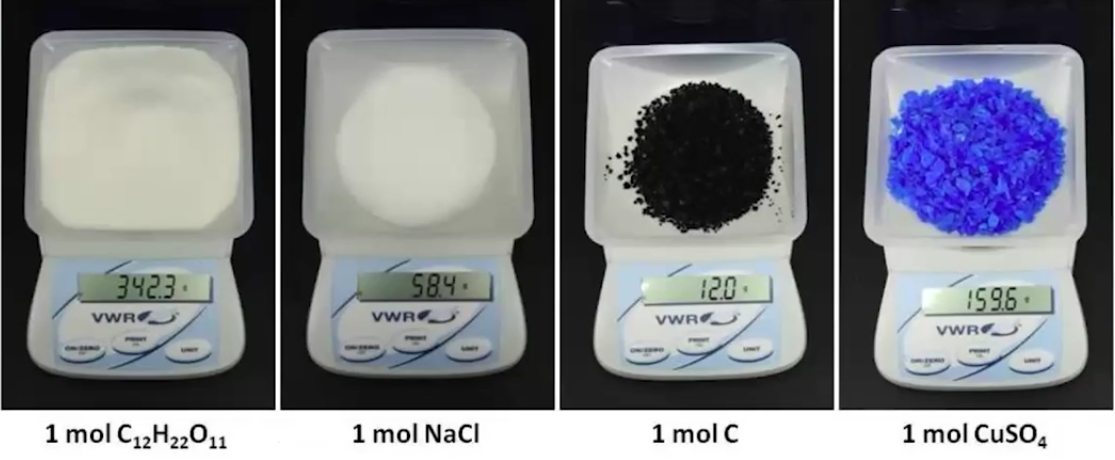
\includegraphics[width=.9\linewidth]{./images/Diagram1.png}
\caption{\label{fig:1}Compounds (\(\ce{C12H22O11},\ \ce{NaCl},\ \ce{C},\ \ce{CuSO4}\))}
\end{figure}

All \(4\) samples in figure 1 contain \(1\) mol. That means each sample has
\(6.02214129 × 10^{23}\) particles. If we were to write that number every
time we do a calculation, it would be needlessly tedious. Moles help link
between the micro world of atoms and molecules to the macro world of grams
and kilograms.

\subsection{How do we find the mass of sucrose (\(\ce{C12H22O11}\))?}
\label{sec:orga4cdada}
\begin{enumerate}
\item Count atoms in chemical formula
\begin{itemize}
\item We have \(12\) carbon atoms, \(22\) hydrogen atoms, and \(11\) oxygen atoms
\end{itemize}
\item Find the atomic mass of each element 
\begin{itemize}
\item \(\text{Carbon}=12.01u,\ \text{Hydrogen} = 1.01u,\ \text{Oxygen} = 16.00u\)
\end{itemize}
\item Multiply atoms by atomic mass of each element, to find total mass
\begin{enumerate}
\item \(C = 12*12.01 = 144.12u\)
\item \(H = 22*1.01 = 22.22u\)
\item \(O = 11*16.00u = 176.00u\)
\end{enumerate}
\item Find the total
\begin{itemize}
\item \(Total = 144.14 + 22.22 + 176.00 = 342.3u\)
\end{itemize}
\end{enumerate}

However, we still don't have the correct answer. Thats because \(1\
   molecule\neq1\ mol\). The mass of each sample is equal to the formula mass of
one particle in the units of grams. This is the molar mass

(Above, u = g/mol)

\subsection{Example 1}
\label{sec:org017097c}
What is the molar mass of \(\ce{H2SO4}\)?
\begin{enumerate}
\item Count the atoms (\(2\) hydrogen, \(1\) Sulfur, \(4\) Oxygen)
\item Find the atomic mass of each element 
\begin{enumerate}
\item \(H = 1.01u\)
\item \(S = 32.06u\)
\item \(O = 16.00u\)
\end{enumerate}
\item Multiply it out 
\begin{enumerate}
\item \(H = 2*1.01 = 2.02u\)
\item \(S = 1*32.06 = 32.06u\)
\item \(O = 4*16.00 = 64.00u\)
\end{enumerate}
\item Add the results 
\begin{itemize}
\item \(2.02u + 32.06u + 64.00y = 98.08u\)
\end{itemize}
\item Use the correct units for molar mass 
\begin{itemize}
\item \(= 98.08 g/mol\)
\end{itemize}
\end{enumerate}

\subsection{Example 2}
\label{sec:org70b76e3}
What is the molar mass of \(\ce{Al(NO3)3}\)?
\begin{enumerate}
\item Count the atoms (\(1\) Aluminium, \(3\) Nitrogen, \(9\) Oxygen)
\item Find the atomic mass of each element 
\begin{enumerate}
\item \(Al = 26.98u\)
\item \(N = 14.01u\)
\item \(O = 16.00u\)
\end{enumerate}
\item Multiply it out 
\begin{enumerate}
\item \(Al = 26.98u * 1 = 26.98u\)
\item \(N = 14.01u * 3 = 42.03u\)
\item \(O = 16.00u * 9 = 144.0u\)
\end{enumerate}
\item Add the results
\begin{itemize}
\item \(26.98 + 42.03 + 144.0u = 213.01u\)
\end{itemize}
\item Use the correct units for molar mass 
\begin{itemize}
\item \(= 213.01 g/mol\)
\end{itemize}
\end{enumerate}

\section{1.1 Daily 2 - Moles and Molar Mass}
\label{sec:orgd56c3a7}
\end{document}
